\documentclass[12pt,a4paper]{report}
\usepackage[utf8]{inputenc}
\usepackage[utf8]{vietnam} %Bien dich duoc tieng Viet
\usepackage{amsmath,amsfonts,amssymb} %Font toan
\usepackage{type1cm}
\usepackage{graphicx}
%\graphicspath{ {images/} }
\usepackage{subfig}
\usepackage[unicode]{hyperref} %Tu dong tao bookmark
\usepackage{indentfirst} %Thut vao dau dong o tat ca cac doan
\usepackage{listings} %Dinh dang code
\usepackage{color} %Mau sac
\usepackage[left=3cm,right=3cm,top=2.5cm,bottom=2.5cm]{geometry} %Canh lề trái - phải - trên - dưới cho tài liệu
\definecolor{dkgreen}{rgb}{0,0.6,0}
\definecolor{gray}{rgb}{0.5,0.5,0.5}
\definecolor{mauve}{rgb}{0.58,0,0.82}

\lstset{frame=tb,
  language=C,
  aboveskip=3mm,
  belowskip=3mm,
  showstringspaces=false,
  columns=flexible,
  basicstyle={\small\ttfamily},
  numbers=left,
  numberstyle=\tiny\color{gray},
  keywordstyle=\color{blue},
  commentstyle=\color{dkgreen},
  stringstyle=\color{mauve},
  breaklines=true,
  captionpos=t,
  breakatwhitespace=true,
  tabsize=2
}
\begin{document}
%\input{title-page.tex}
%\input{install-pi/Install-Pi-OS.tex}
\tableofcontents
\chapter{Cài đặt hệ điều hành cho Raspberry Pi}
\section{Chuẩn bị}
\subsection{Phần cứng}
\begin{list}{--}{}
\item Máy tính Raspberry Pi: bạn có thể sử dụng Model $A$, $B$, $A+$, $B+$, $Pi~2$, $Pi~3$, $Pi Zero$.
\begin{figure}[!h]
\begin{center}
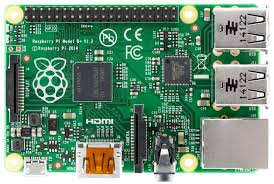
\includegraphics[scale=.5]{setup-os/images/Pi-H}
\end{center}
\caption{Raspberry Pi model B+}
\end{figure}
\item Thẻ nhớ SD: Dung lượng 4GB trở lên, tốc độ cao. Nên sử dụng thẻ nhớ có dung lượng $8GB$. Có thể sử dụng thêm Adapter (tùy theo phiên bản Pi mà bạn sử dụng).
\begin{figure}[!h]
\begin{center}
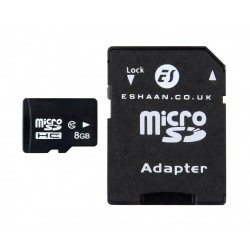
\includegraphics[scale=.4]{setup-os/images/SD-H}
\end{center}
\caption{Thẻ nhớ SD và Adapter}
\end{figure}
\item Nguồn điện cấp cho Pi hoạt động: nguồn DC $5V-1A$
\item Các ngoại vi khác: dây kết nối HDMI (hoặc cáp VGA và cáp chuyển đổi HDMI to VGA), màn hình có cổng HDMI (hoặc hoặc màn hình có cổng VGA), chuột, bàn phím, dây kết nối mạng.
\item[$\ast$] Nếu không có các thiết bị ngoại vi trên thì sử dụng các loại cáp truyền nhận dữ liệu giữa Pi và máy tính cũng có thể thực hiện được, ví dụ: RS232, PL2303.
\end{list}
\subsection{Phần mềm}
\begin{list}{--}{}
\item Phần mềm Format thẻ nhớ, ví dụ: SDFormatter.

Địa chỉ: \verb|https://www.sdcard.org/downloads/formatter_4/|
\item Phần mềm ghi hệ điều hành vào thẻ nhớ, ví dụ: Win32DiskImage.

Địa chỉ: \verb|https://sourceforge.net/projects/win32diskimager/|
\item Hệ điều hành: Chọn một trong hai hệ điều hành sau để tải về máy.
\begin{list}{+}{}
\item Trong phần này mình sử dụng hệ điều hành Raspbian.

Địa chỉ: \verb|https://www.raspberrypi.org/downloads/raspbian/|

\item Cài đặt bằng NOOBS: tích hợp nhiều hệ điều hành vào một gói, bạn thích sử dụng hệ điều hành nào thì chọn hệ điều hành đó.

Địa chỉ: \verb|https://www.raspberrypi.org/downloads/noobs/|
\end{list}
\end{list}
\section{Cài đặt hệ điều hành}
Bạn chọn một trong các cách sau để cài đặt.
\subsection{Cài đặt hệ điều hành Raspbian}
\begin{list}{--}{}
\item Cài đặt các phần mềm ở phần chuẩn bị, ví dụ: \verb|SDFormatter| và \verb|Win32DiskImage|.
\item Giải nén thư mục chứ hệ điều hành Raspbian (file .zip) được file \verb|.img|.
\item Mở phần mềm \verb|SDFormatter|, định dạng lại thẻ nhớ chuẩn bị ghi hệ điều hành lên. Chọn \verb|Format|. Thông báo xuất hiện chọn YES.
\begin{figure}[!h]
\begin{center}
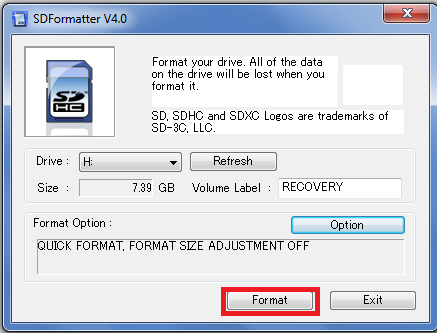
\includegraphics[scale=.4]{setup-os/images/SDFormatter}
\end{center}
\caption{Format lại thẻ nhớ để cài đặt hệ điều hành}
\end{figure}
\item Mở phần mềm \verb|Win32DiskImage| để ghi hệ điều hành vào thẻ nhớ, chọn đường dẫn đến file \verb|.img| đã giải nén ở bước trên. Chọn \verb|Write|. Thông báo xuất hiện chọn YES.
\begin{figure}[!h]
\begin{center}
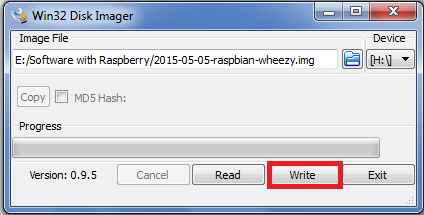
\includegraphics[scale=.5]{setup-os/images/Win32DiskImage}
\end{center}
\caption{Ghi hệ điều hành vào thẻ nhớ}
\end{figure}
\item Đợi cho quá trình ghi hệ điều hành hoàn thành là được.
\item Gắn thẻ nhớ vào Pi, kết nối màn hình, chuột, bàn phím, cấp nguồn khởi động và tiến hành một số cài đặt cần thiết khác.
\end{list}
\subsection{Cài đặt hệ điều hành Raspbian bằng NOOBS}
Khi cài đặt hệ điều hành bằng bản NOOBS, nó cũng có chứa hệ điều hành Raspbian, bạn có thể cài đặt hệ điều hành Raspbian bằng cách này.\\

Muốn có nhiều hệ điều hành khác được chọn thì bạn cần có kết nối Internet (sử dụng dây LAN).
\begin{list}{--}{}
\item Cài đặt các phần mềm ở phần chuẩn bị, ví dụ: \verb|SDFormatter| (không cần sử dụng phần mềm ghi hệ điều hành).
\item Giải nén thư mục chứa hệ điều hành trong bản NOOBS (file .zip).
\item Mở phần mềm \verb|SDFormatter|, định dạng lại thẻ nhớ chuẩn bị chép hệ điều hành lên. Chọn \verb|Format|. Thông báo xuất hiện chọn YES.
\begin{figure}[!h]
\begin{center}
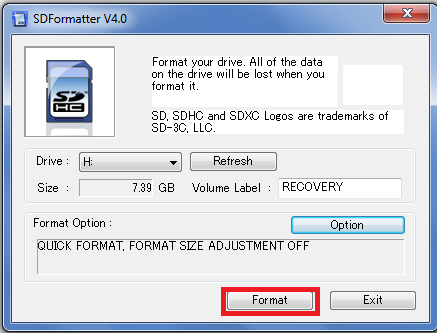
\includegraphics[scale=.4]{setup-os/images/SDFormatter}
\end{center}
\caption{Format lại thẻ nhớ để cài đặt hệ điều hành}
\end{figure}
\item Copy toàn bộ nội dung trong thư mục đã giải nén ở trên (của bản NOOBS) vào thẻ nhớ.
\item Gắn thẻ nhớ vào Pi, kết nối màn hình, chuột và bàn phím (hoặc các phương pháp tương đương khác), sẽ có một danh sách các hệ điều hành được được ra, bạn chọn hệ điều hành muốn cài đặt rồi nhấn \verb|Install| sau đó đợi quá trình cài đặt xong, khởi động lại Pi là hoàn thành.
\begin{figure}[!h]
\begin{center}
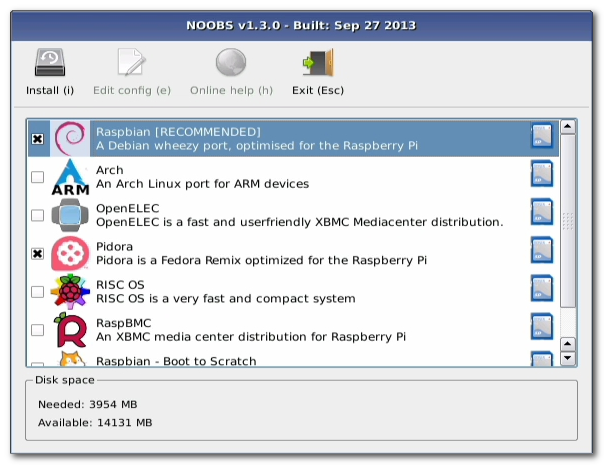
\includegraphics[scale=.5]{setup-os/images/NOOBS}
\end{center}
\caption{Các hệ điều hành trong bản NOOBS}
\end{figure}
\item Sau khi cài đặt hệ điều hành xong, tiến hành một số cài đặt cần thiết khác.
\end{list}
\section{Thiết lập ban đầu cho Raspberry Pi}
Sau khi cài đặt và khởi động, bạn có thể muốn thiết lập lại các cài đặt mặc định của hệ điều hành sao cho phù hợp với bạn. Sau khi thiết lập xong, reset lại Pi: \verb|sudo reboot|\\

Thực hiện lệnh: \verb|sudo raspi-config| để tiến hành cài đặt. Các tùy chọn thiết lập như hình dưới:
\begin{figure}[!h]
\begin{center}
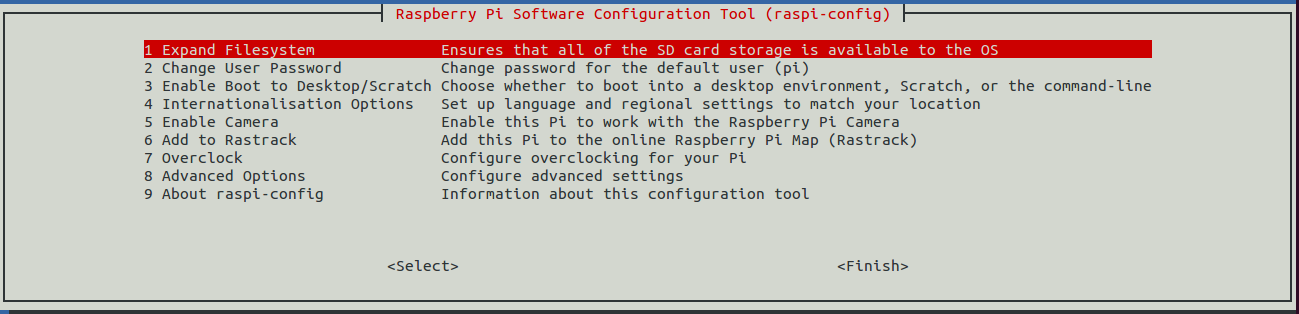
\includegraphics[scale=.35]{setup-os/images/raspi}
\end{center}
\caption{Các tùy chọn thiết lập cho Pi}
\end{figure}
\subsection{Thiết lập ngôn ngữ, múi giờ và kiểu bàn phím}
Thay đổi ngôn ngữ, múi giờ, kiểu bàn phím: \verb|Internationalisation Options|, được các lựa chọn sau:
\begin{figure}[!h]
\begin{center}
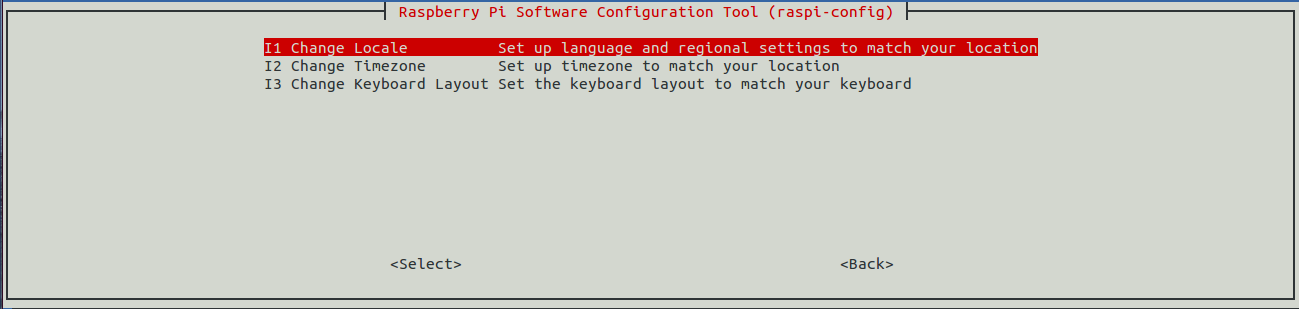
\includegraphics[scale=.35]{setup-os/images/Time}
\end{center}
\caption{Các tùy chọn thiết lập ngôn ngữ, múi giờ, kiểu bàn phím}
\end{figure}
\begin{list}{--}{}
\item Chọn \verb|Change Locale|: để thay đổi ngôn ngữ.

Đổi \verb|en_GB.UTF-8 UTF-8| thành \verb|en_US.UTF-8 UTF-8 | (sử dụng dấu cách \verb|space| để chọn hoặc bỏ chọn).
\begin{figure}[!h]
\begin{center}
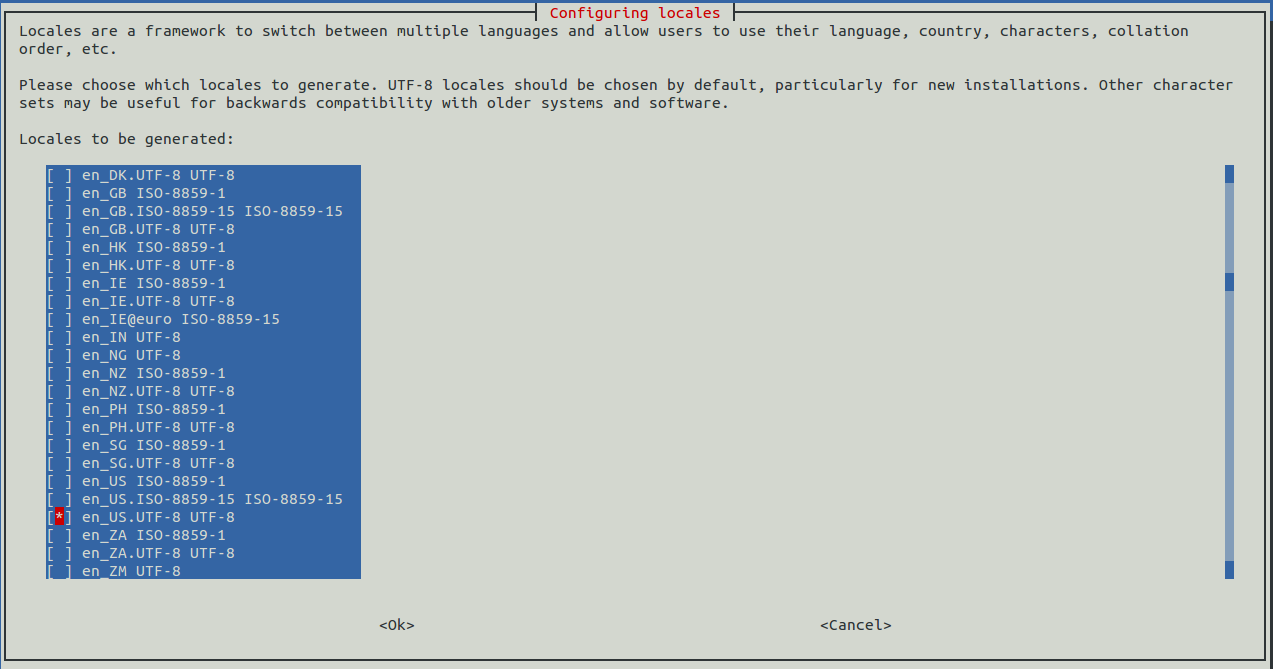
\includegraphics[scale=.35]{setup-os/images/lang}
\end{center}
\caption{Thay đổi ngôn ngữ thành \textsf{en\_US.UTF-8 UTF-8}}
\end{figure}
\item Chọn \verb|Change TimeZone|: để thay đổi múi giờ.

Chọn \verb|Asia| rồi chọn tiếp \verb|Ho_Chi_Minh|.
\begin{figure}[!h]
\begin{center}
\subfloat[Chọn \textsf{Asia}]
  {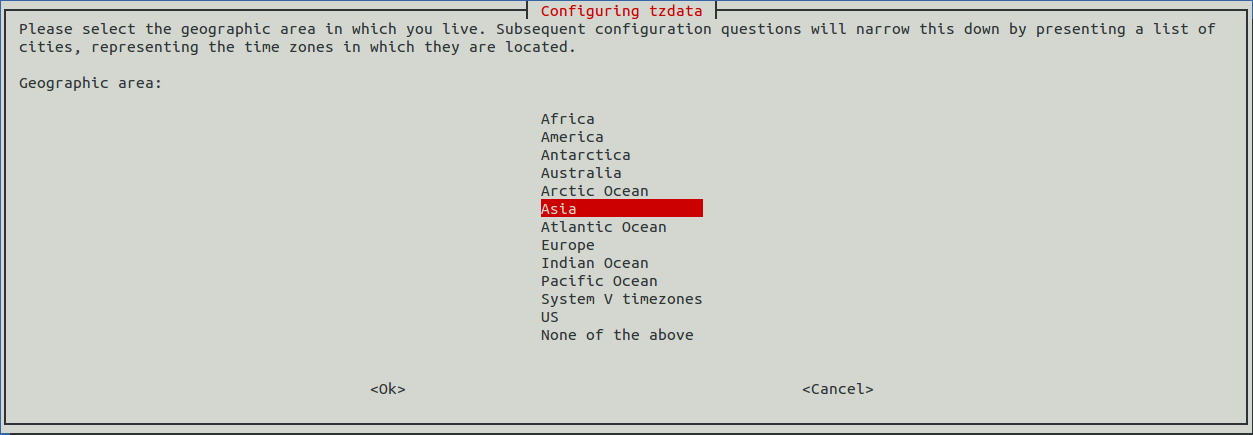
\includegraphics[scale=.35]{setup-os/images/time-zone}}\\
\subfloat[Chọn \textsf{Ho\_Chi\_Minh}]
  {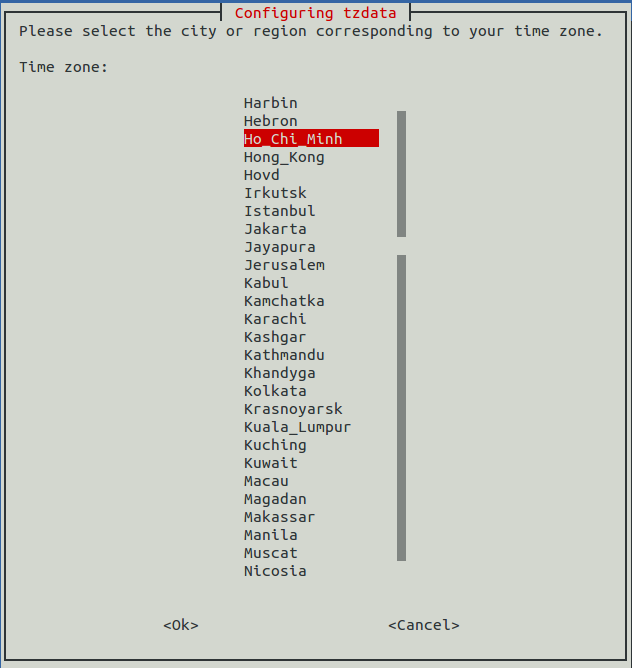
\includegraphics[scale=.35]{setup-os/images/time-zone-2}}
\end{center}
\caption{Thay đổi múi giờ}
\end{figure}
\newpage
\item Thay đổi kiểu bàn phím, dùng lệnh:
\begin{lstlisting}[language=bash]
$ sudo nano /etc/default/keyboard
\end{lstlisting}
Nội dung file như sau:
\begin{lstlisting}[language=bash]
# KEYBOARD CONFIGURATION FILE

# Consult the keyboard(5) manual page.

XKBMODEL="pc105"
XKBLAYOUT="gb"
XKBVARIANT=""
XKBOPTIONS=""

BACKSPACE="guess"
\end{lstlisting}

Đổi các khai báo sau: \verb|pc105| thành \verb|pc104| và \verb|gb| thành \verb|us|, sau khi thay đổi nội dung như sau:
\begin{lstlisting}[language=bash]
# KEYBOARD CONFIGURATION FILE

# Consult the keyboard(5) manual page.

XKBMODEL="pc104"
XKBLAYOUT="us"
XKBVARIANT=""
XKBOPTIONS=""

BACKSPACE="guess"
\end{lstlisting}

Nhấn \verb|Ctrl + X + Y| và \verb|Enter| để lưu nội dung thay đổi.
\item[$\ast$] Để thoát khỏi \verb|raspi-config| nhấn phím \verb|Esc|.
\end{list}
\subsection{Cập nhật Raspberry Pi}
\begin{list}{--}{}
\item Kiểm tra cập nhật:
\begin{lstlisting}[language=bash]
$ sudo apt-get update
\end{lstlisting}
\item Tiến hành cập nhật:
\begin{lstlisting}[language=bash]
$ sudo apt-get upgrate
\end{lstlisting}
Nếu có các thay đổi bạn cần chọn \verb|Y| để bắt đầu cặp nhật.
\item Cập nhật \verb|firmware|:
\begin{lstlisting}[language=bash]
$ sudo rpi-update
\end{lstlisting}
\end{list}
\subsection{Thiết lập dòng cung cấp cho ngõ ra USB}
Dòng mặc định là $600mA$, cần tăng dòng lên $1200mA$ để sử dụng các USB.
\begin{list}{--}{}
\item Mở file \verb|config.txt| để thay đổi nội dung:
\begin{lstlisting}[language=bash]
$ sudo nano /boot/config.txt
\end{lstlisting}
\item Thêm nội dung sau vào cuối file \verb|config.txt| (dùng \verb|Ctrl + V| để di chuyển nhanh):
\begin{lstlisting}[language=bash]
max_usb_current=1
\end{lstlisting}
Nhấn \verb|Ctrl + X + Y| để lưu thay đổi.
\end{list}
\subsection{Bật SSH}
\verb|SSH| cho phép điều khiển Pi từ xa thông qua mạng Internet.
\begin{list}{--}{}
\item Chọn \verb|Advanced Options|: hình \ref{Fig:Advanced Options}.
\begin{figure}[!h]
\begin{center}
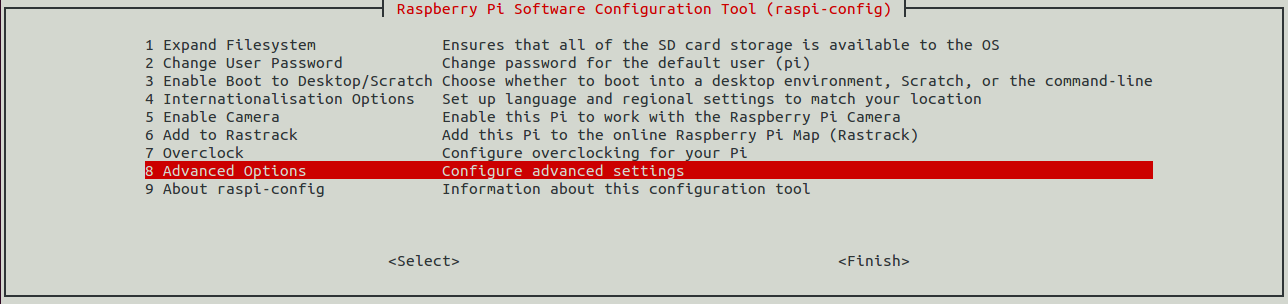
\includegraphics[scale=.35]{setup-os/images/ssh-setup}
\end{center}
\caption{Mở các tùy chọn nâng cao \textsf{Advanced Options}}\label{Fig:Advanced Options}
\end{figure}
\item Chọn \verb|A4 SSH|: hình \ref{Fig:A4 SSH}.
\begin{figure}[!h]
\begin{center}
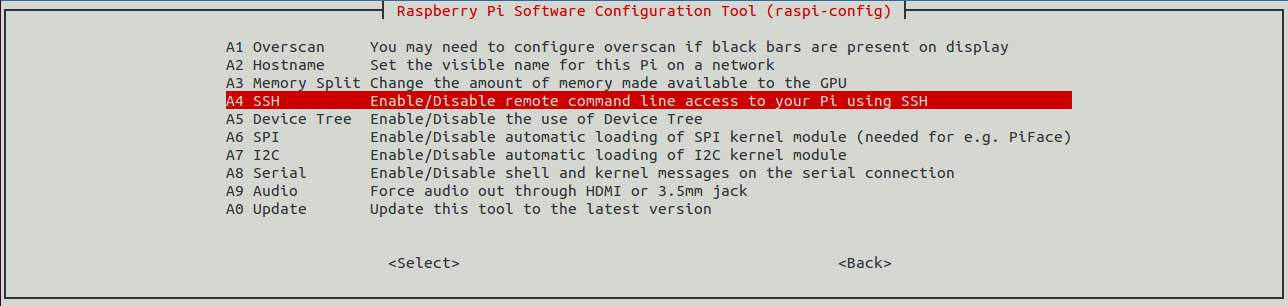
\includegraphics[scale=.35]{setup-os/images/a4-ssh}
\end{center}
\caption{Chọn  \textsf{A4 SSH}}\label{Fig:A4 SSH}
\end{figure}
\item Chọn \verb|Enable|: hình \ref{Fig:Enable}.
\begin{figure}[!h]
\begin{center}
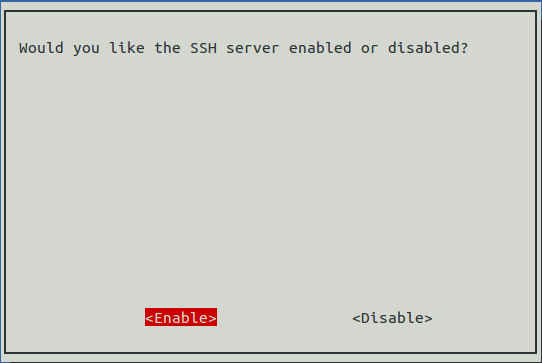
\includegraphics[scale=.35]{setup-os/images/a4-ssh-2}
\end{center}
\caption{Chọn \textsf{Enable}}\label{Fig:Enable}
\end{figure}
\end{list}
\chapter{Điều khiển và sao chép dữ liệu với Raspberry Pi}
%Có một cách có thể dùng để điều khiển Raspberry Pi
\section{Điều khiển bằng cách kết nối trực tiếp với màn hình, bàn phím và chuột}
\begin{itemize}
\item \textit{Điều khiển}: Kết nối chuột và bàn phím qua các cổng USB. Với màn hình thông thường có 2 loại: màn hình hỗ trợ cổng HDMI và màn hình hổ trợ cổng VGA.
\item \textit{Sao chép dữ liệu}: Sử dụng USB.
\end{itemize}
\subsection{Màn hình hổ trợ cổng HDMI}
Ta kết nối màn hình qua cable HDMI. Có thể bạn sẽ cần tùy chỉnh một số thông sau cho phù hợp:
\subsection{Màn hình hổ trợ cổng VGA}
Để hiển thị được, ta cần có cable chuyển đồi từ VGA sang HDMI.
\begin{figure}[!h]
\begin{center}
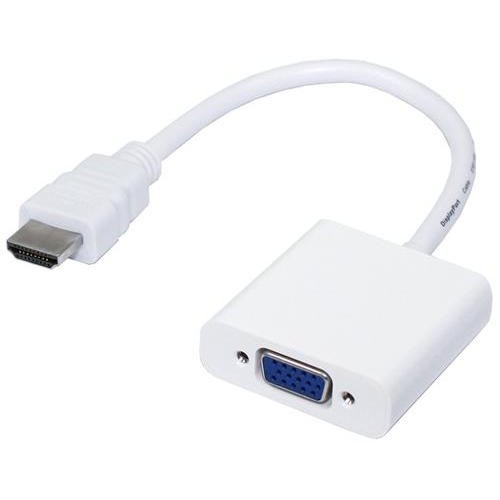
\includegraphics[scale=.3]{remote/images/HDMI-VGA-white}
\end{center}
\caption{Cáp chuyển đổi từ cổng HDMI sang cổng VGA}
\end{figure}
\section{Điều khiển bằng giao tiếp nối tiếp thông qua cổng RS232} \label{Sec:rs232}
Khi kết nối bằng module RS232, cần cấp nguồn cho Pi hoạt động.
\begin{figure}[!h]
\begin{center}
\subfloat[Module RS232 to TTL]
  {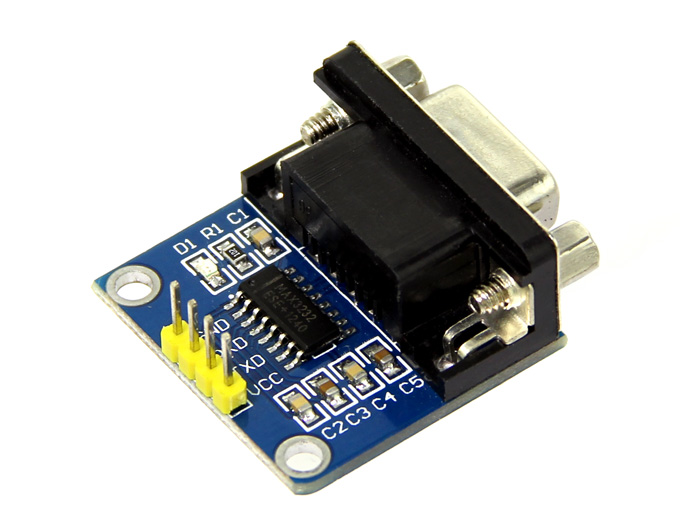
\includegraphics[width=.3\linewidth]{remote/images/RS232-to-ttl}}\hspace{1cm}
\subfloat[Cáp USB to COM]
  {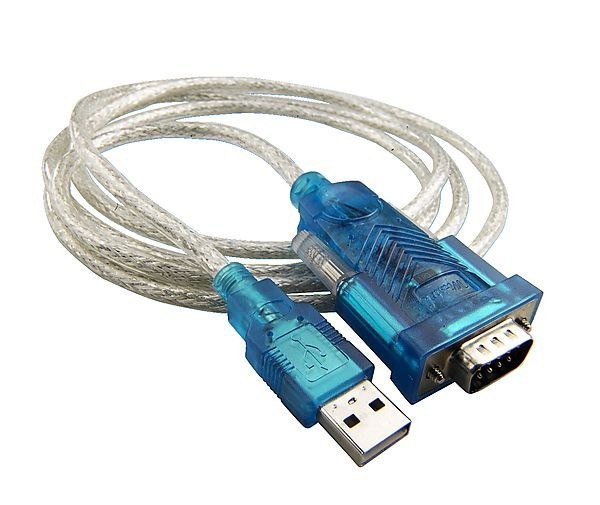
\includegraphics[width=.3\linewidth]{remote/images/cap-usb-to-com}}
\end{center}
\caption{Module RS232 to TTL và Cáp USB to COM}
\end{figure}
\begin{itemize}
\item Thực hiện kết nối Pi và module RS232 như sau:
\begin{center}
\begin{tabular}{c|c}
Pi & RS232\\ \hline
3.3V & VCC\\
TX & TX \\ 
RX & RX\\
GND & GND
\end{tabular}
\end{center}
\item Cài đặt gói phần mềm \verb|screen|: \verb|sudo apt-get install screen| trên máy tính Ubuntu.
\item Chạy lệnh sau: \verb|sudo screen /dev/ttyUSB0 115200|
\item Thực hiện xong lệnh trên, ta nhấn Enter một lần nữa để kết nối với Pi.
\item Nhập username và password để đăng nhập.
\item Sao chép dữ liệu: dùng USB.
\item[$\ast$] Ta có thể dùng Putty (trên hệ điều hành Window) để điều khiển: chọn \verb|Serial|, điền vào khung \verb|Serial line| tên cổng (ví dụ: COM1, COM2,\ldots), trong khung \verb|Speed| điền tốc độ là \verb|115200|. Nhập username và password để đăng nhập.
\end{itemize}
\section{Điều khiển bằng giao tiếp nối tiếp thông qua cáp USB to COM PL2303}
Khi kết nối bằng cáp USB to COM PL2303 thì không cần cấp nguồn ngoài cho Pi hoạt động (do Pi sẽ lấy nguồn từ cổng USB thông qua cáp).
\begin{figure}[!h]
\begin{center}
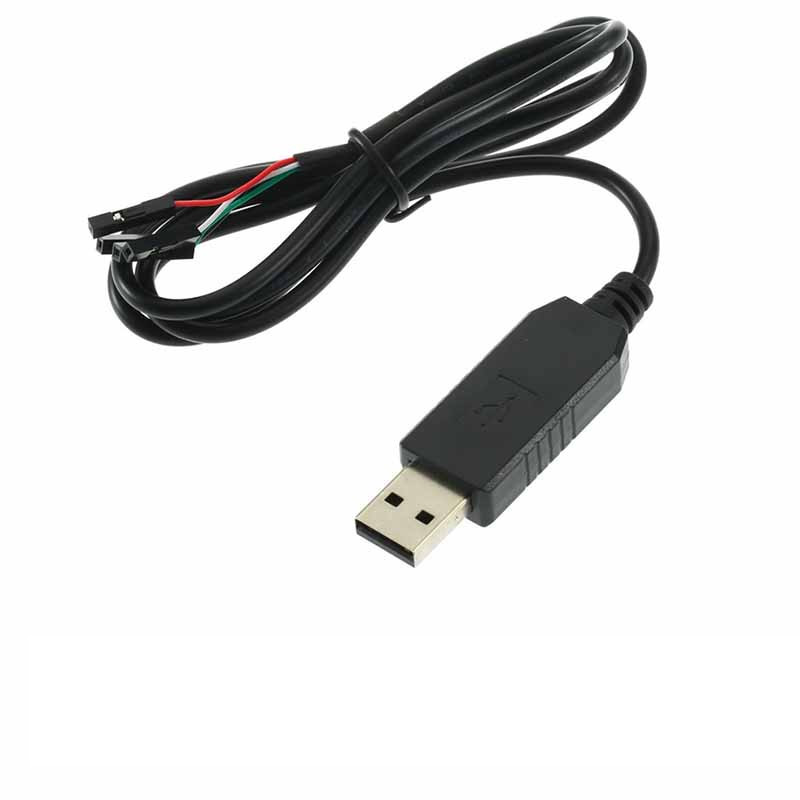
\includegraphics[scale=.3]{remote/images/cap-usb-to-com-pl2303}
\end{center}
\caption{Cáp USB to COM PL2303}
\end{figure}
\begin{itemize}
\item Thực hiện kết nối Pi và cáp USB to COM PL2303 như sau:
\begin{center}
\begin{tabular}{c|c|c}
Pi & PL2303 & Màu dây\\ \hline
5V & VCC & Đỏ\\
TX & RX & Trắng\\ 
RX & TX & Xanh\\
GND & GND & Đen
\end{tabular}
\end{center}
\item Phần cài đặt và điều khiển tương tự như cổng RS232 (xem \textit{mục \ref{Sec:rs232} trang \pageref{Sec:rs232}}).
\end{itemize}
\section{Điều khiển từ xa khi Raspberry Pi có kết nối mạng}
Khi Raspberry Pi có kết nối mạng Internet, ta có thể dùng các phần mềm: \verb|SSH|, \verb|Remote Desktop|, \verb|VNC|,\ldots~ để điều khiển.
\begin{itemize}
\item Kiểm tra địa chỉ IP của Pi bằng phần mềm: ipscan (trên Windows) hoặc nmap (trên Ubuntu).
\begin{itemize}
\item Phần mềm \verb|ipscan|: giao diện trực quan, dễ sử dụng.
\item Chương trình \verb|nmap| trên Ubuntu:
\begin{list}{+}{}
\item Cài đặt chương trình:
\begin{lstlisting}[language=bash]
sudo apt-get install nmap
\end{lstlisting}
\item Tìm các địa chỉ IP trong mạng nội bộ:
\begin{lstlisting}[language=bash]
sudo nmap -sP 192.168.1.1-254
\end{lstlisting}
THay đổi địa chỉ IP \verb|192.168.1.1| cho phụ hợp với địa chỉ IP của bạn.
\end{list}
\end{itemize}
\item Chọn chương trình phù hợp để điều khiển Raspberry Pi: 
\begin{itemize}
\item Với \verb|SSH|: không hổ trợ giao diện đồ họa.
\begin{lstlisting}[language=bash]
ssh pi@192.168.0.100
\end{lstlisting}
Trong đó: \verb|pi| là tên user bạn cần đăng nhập, kế tiếp là địa chỉ IP của Raspberry Pi.
\item Với \verb|VNC| hoặc \verb|Remote Desktop|: có hổ trợ giao diện đồ họa.
\item[$\ast$]  Với \verb|Remote Desktop| Pi cần cài đặt \verb|xrdp|:
\begin{lstlisting}[language=bash]
sudo apt-get install xrdp
\end{lstlisting}
\end{itemize}
\item Tùy theo chương trình bạn chọn: ta cần phải nhập địa chỉ IP, username và password (nếu có yêu cầu điền số \verb|port|: ta điền 22).
\item Sao chép dữ liệu:
\begin{itemize}
\item Trên Window: dùng \verb|Winscp|.
\item Trên Ubuntu: dùng \verb|FileZilla|.
\begin{figure}[!h]
\begin{center}
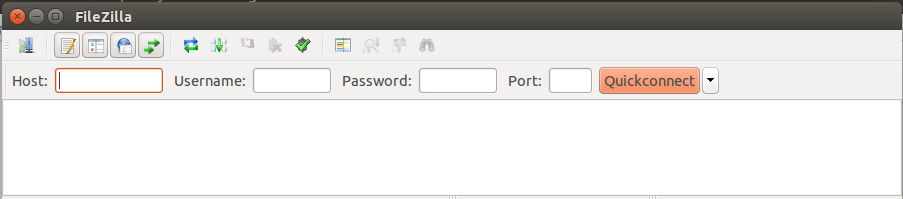
\includegraphics[scale=.45]{remote/images/FileZilla}
\end{center}
\caption{Sao chép dữ liệu từ Raspberry Pi với FileZilla}
\end{figure}
\begin{list}{+}{}
\item \verb|Host|: điền địa chỉ IP.
\item \verb|Username|: tên cần đăng nhập.
\item \verb|Password|: mật khẩu đăng nhập cho tài khoản ở ô \verb|Username|.
\item \verb|Port|: điền số 22.
\end{list}
\item[$\ast$] Ta cũng cần nhập vào thông tin như trên để truy cập được Pi.
\end{itemize}
\item \textit{Lưu ý}: Phần trình bày trên áp ngay cho mạng nội bộ, khi không phải mạng nội bộ ta cần cấu hình mạng rồi mới áp dụng được hướng dẫn ở phần này.
\end{itemize}

\chapter{Mạng Internet với Raspberry Pi}
\section{Kết nối internet với dây mạng LAN}
Trên Raspberry Pi có hổ trợ cổng Ethernet, chúng ta có thể kết nối dây mạng trực tiếp vào đây.
\section{Kết nối internet với USB Wifi}
Trong phần này, mình sử dụng USB Wifi TP Link 725N
\subsection{Cài đặt Drive}
Tham khảo tại: \verb|https://www.raspberrypi.org/forums/viewtopic.php?p=462982|

Thực hiện theo các bước sau:
\begin{itemize}
\item Xác định phiên bản hệ điều hành Raspbain:
\begin{lstlisting}[language=make]
$ uname -a
Linux raspberrypi 4.1.13+ #826 PREEMPT Fri Nov 13 20:13:22 GMT 2015 armv6l GNU/Linux
\end{lstlisting}
Trong ví dụ trên, phiên bản hệ điều hành là \verb|4.1.13+ #826|. 
\item Vào địa chỉ bên dưới để tải drive:

\verb|https://www.raspberrypi.org/forums/viewtopic.php?p=462982|
\item Cài đặt drive, thực hiện các lệnh bên dưới:
\begin{lstlisting}[language=make]
wget https://dl.dropboxusercontent.com/u/80256631/8188eu-201xyyzz.tar.gz
tar -zxvf 8188eu-201xyyzz.tar.gz
sudo install -p -m 644 8188eu.ko /lib/modules/$(uname -r)/kernel/drivers/net/wireless
sudo insmod /lib/modules/$(uname -r)/kernel/drivers/net/wireless/8188eu.ko
sudo depmod -a
\end{lstlisting}
Đối với Raspberry Pi 2, chúng ta chỉ cần thực hiện 2 lệnh sau:
\begin{lstlisting}[language=make]
tar xzf 8188eu-2015yyzz.tar.gz
./install.sh
\end{lstlisting}
Với \verb|8188eu-201xyyzz.tar.gz| là drive phù hợp với phiên bản hệ điều hành của bạn.

Bạn có thể tải drive từ máy tính rồi chép vào Raspberry Pi để cài đặt (cách này dùng cho Pi chưa được kết nối với Internet).
\item[$\ast$] Trong quá trình cập nhật các phiên bản mới của hệ điều hành, khi đó Raspberry Pi không còn nhận USB Wifi nữa, lúc đó ta cần cài đặt Drive mới cho USB Wifi.
\end{itemize}
\subsection{Cài đặt địa chỉ IP tĩnh}
Tham khảo tại địa chỉ: 

\begin{footnotesize}
\verb|http://weworkweplay.com/play/automatically-connect-a-raspberry-pi-to-a-wifi-network/|
\end{footnotesize}\\

Ta sửa đổi nội dung của 2 tập tin dưới đây:
\begin{itemize}
\item Tập tin: \verb|interfaces|, mở tập tin:
\begin{lstlisting}[language=bash]
$ sudo nano /etc/network/interfaces
\end{lstlisting}
và thay đổi nội dung như sau:
\lstinputlisting[language=make]{interfaces}
\item Tập tin: \verb|wpa_supplicant.conf|,  mở tập tin:
\begin{lstlisting}[language=bash]
$ sudo nano /etc/wpa_supplicant/wpa_supplicant.conf
\end{lstlisting}
và thay đổi nội dung như sau:
\lstinputlisting[language=make]{wpa_supplicant.conf}
\end{itemize}
\section{Sử dụng chung Wifi với Laptop}
Ta kết nối cổng Ethernet của Pi và Laptop với nhau. Sử dụng tín năng Share Wifi trên Laptop:
\subsection{Hệ điều hành Ubuntu}
Thực hiện theo các bước sau:
\begin{itemize}
\item Trong thanh tìm kiếm \verb|Dash|: gõ vào \verb|Network Connections|, chọn \verb|Network Connections| để mở lên.
\begin{figure}[!h]
\begin{center}
{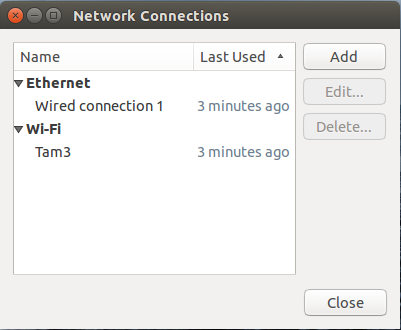
\includegraphics[scale=.5]{network/images/share-wifi-1}}
\end{center}
\caption{Mở \textsf{Network Connections}}
\end{figure}
\item Chọn \verb|Add|:
\begin{figure}[!h]
\begin{center}
{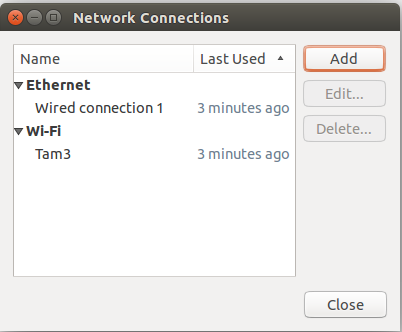
\includegraphics[scale=.5]{network/images/share-wifi-2}}
\end{center}
\caption{Chọn \textsf{Add}}
\end{figure}
\newpage
\item Chọn \verb|Create|:
\begin{figure}[!h]
\begin{center}
{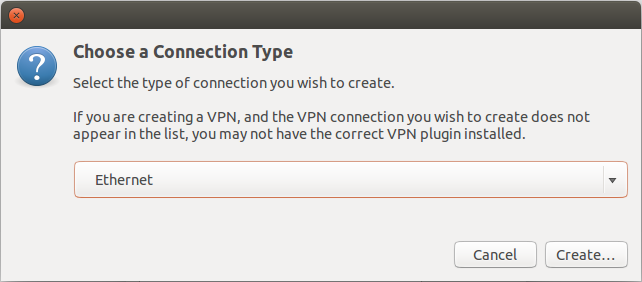
\includegraphics[scale=.4]{network/images/share-wifi-3}}
\end{center}
\caption{Chọn \textsf{Create\ldots}}
\end{figure}
\item Điền tên trong ô \verb|Connection name|:
\begin{figure}[!h]
\begin{center}
{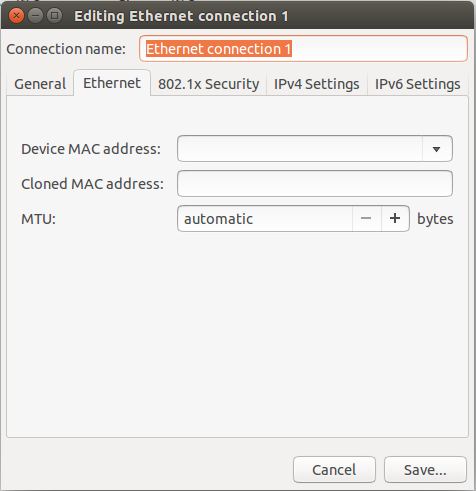
\includegraphics[scale=.4]{network/images/share-wifi-4}}
\caption{Điền tên trong ô \textsf{Connection name}}
\end{center}
\end{figure}
\item Chọn tab \verb|IPv6 Settings|, chọn \verb|Method| là \verb|Automactic|:
\begin{figure}[!h]
\begin{center}
{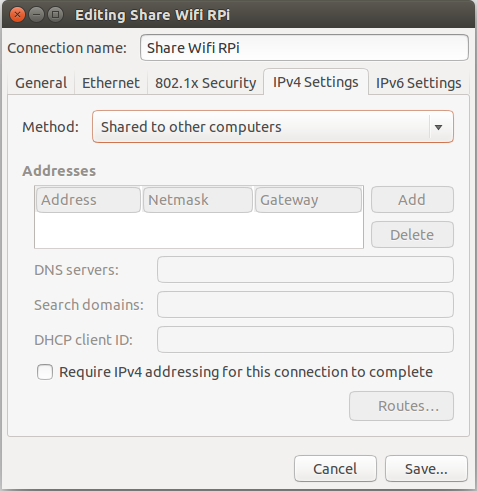
\includegraphics[scale=.4]{network/images/share-wifi-5}}
\caption{Chọn tab \textsf{IPv6 Settings}, chọn \textsf{Method} là \textsf{Automactic}}
\end{center}
\end{figure}
\item Chọn tab \verb|IPv4 Settings|, chọn \verb|Method| là \verb|Share to orther computers|:
\begin{figure}[!h]
\begin{center}
{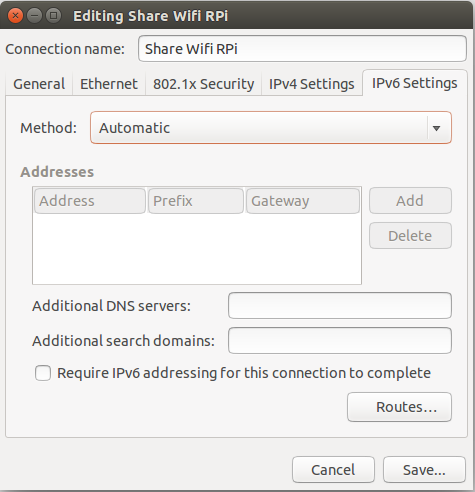
\includegraphics[scale=.5]{network/images/share-wifi-6}}
\caption{Chọn tab \textsf{IPv6 Settings}, chọn \textsf{Method} là \textsf{Share to orther computers}}
\end{center}
\end{figure}
\item Chọn \verb|Save| rồi chọn \verb|Close|.
\item Mở cửa sổ lệnh \verb|Terminal| gõ lệnh:
\begin{lstlisting}[language=bash]
$ sudo cat /var/lib/misc/dnsmasq.leases
1461927547 b8:27:eb:6a:bf:9a 10.42.0.31 raspberrypi ff:eb:6a:bf:9a:00:01:00:01:1c:dd:60:6b:b8:27:eb:6a:bf:9a
\end{lstlisting}
\item Địa chỉ của Pi lúc này là \verb|10.42.0.31|
\item Truy cập qua SSH bằng lệnh:
\begin{lstlisting}[language=bash]
$ ssh pi@10.42.0.31
\end{lstlisting}
\item Nhập password đăng nhập tài khoản username là \verb|pi|.
\end{itemize}
\chapter{Tự động đăng nhập Raspberry Pi sau khi khởi động}
\label{Sub:auto-login}
Tham khảo tại:

\textsf{http://www.raspberrypi-spy.co.uk/2015/02/how-to-autorun-a-python-script-on-raspberry-pi-boot/}
%\begin{footnotesize}
%\verb|http://www.raspberrypi-spy.co.uk/2015/02/how-to-autorun-a-python-script-on-raspberry-pi-boot/|
%\end{footnotesize}

Mặc định khi Raspberry Pi khởi động, cần phải đăng nhập username và password mới sử dụng được. Với một số ứng dụng thực tế, cần tự động đăng nhập mới có thể hoạt động được.\\

Thực hiện theo các bước sau:
\begin{itemize}
\item Mở file \verb|inittab|, dùng lệnh:
\begin{lstlisting}[language=bash]
$ sudo nano /etc/inittab
\end{lstlisting}
\item Tìm đến dòng dưới và thêm dấu \verb|#| vào trước nó:
\begin{lstlisting}[language=bash]
1:2345:respawn:/sbin/getty 115200 tty1
\end{lstlisting}
(tìm đến dòng có \verb|1:2345:respawn:/sbin/getty ....| là được, còn các tham số phía sau tùy thuộc vào phiên bản hệ điều hành).
\item Thay thế dòng trên bằng dòng sau (với \verb|pi| là tên username):
\begin{lstlisting}[language=bash]
1:2345:respawn:/bin/login -f pi tty1 </dev/tty1 >/dev/tty1 2>&1
\end{lstlisting}
\item Nhấn \verb|Ctrl - X - Y| để lưu lại nội dung thay đổi và thoát.
\item Khởi động lại Pi: \verb|sudo reboot|.
\end{itemize}
\chapter{Chạy chương trình Python trên Raspberry Pi}
\section{Python trên Raspberry Pi}\label{run-python}
Ta phân biệt theo 2 trường hợp sau:
\begin{itemize}
\item Chạy các lệnh không liên quan đến phần cứng là các chân GPIO, ta sẽ gõ các lệnh sau:
\begin{itemize}
\item Chạy ở chế độ dòng lệnh:
\begin{lstlisting}[language=bash]
$ python
\end{lstlisting}
\item Khi đã có sẳn một file \verb|.py| (ví dụ: \verb|file.py|):
\begin{lstlisting}[language=bash]
$ python file.py
\end{lstlisting}
\end{itemize}
\item Các lệnh liên quan đến phần cứng can thiệp vào các chân GPIO hoặc cần quyền root, ta phải chạy với quyền root: dùng \verb|sudo python| hoặc \verb|sudo python file.py| (cách dùng 2 lệnh này giống như trên).
\end{itemize}
\section{Tự động chạy một chương trình python sau khi Reboot}
Ở phần~\ref{run-python}, ta phải thực hiện đánh lệnh thì file python mới được gọi, với nhiều ứng dụng tự động, cần tự động chạy chương trình python sau khi reboot. Ta có một số cách sau:

Ví dụ, ta cần chạy file python có tên là \verb|myfile.py|.
\subsection{Sử dụng cron}
Tham khảo tại: \verb|https://www.youtube.com/watch?v=8iU9TnYFOV0|\\
Thực hiện theo các bước sau:
\begin{itemize}
\item Không cần tự động đăng nhập.
\item Copy file \verb|myfile.py| đến thư mục \verb|\home\pi| (dùng lệnh \verb|cp|).
\item Mở file \verb|crontab| gõ lệnh:
\begin{lstlisting}[language=bash]
$ sudo crontab -e
\end{lstlisting}
\item Thêm dòng sau vào cuối file: 
\begin{lstlisting}[language=bash]
@reboot sudo python myfile.py &
\end{lstlisting}
Ký hiệu \verb|&| có nghĩa là file \verb|myfile.py| sẽ chạy nền.
\begin{figure}[h!]
\begin{center}
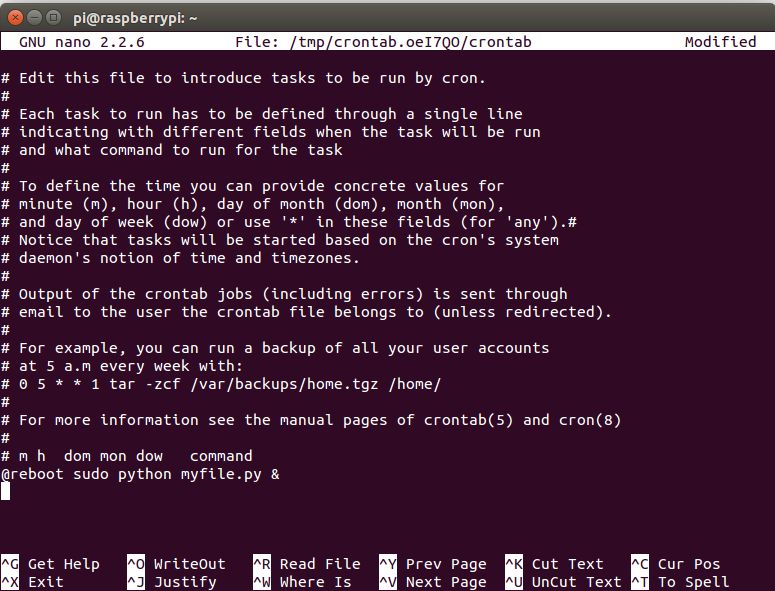
\includegraphics[scale=.5]{run-script-python/images/auto-run-python-1}
\end{center}
\end{figure}
\item Nhấn \verb|Ctrl - X - Y| để lưu lại nội dung thay đổi và thoát.
\item Khởi động lại Pi: \verb|sudo reboot|.
\end{itemize}
Nói thêm về \verb|cron|\footnote{\textsf{https://embeddedday.com/projects/raspberry-pi/a-step-further/running-python-script-at-boot/}} \verb|cron| là một lịch trình, được khai báo với cú pháp sau:
\begin{lstlisting}[language=bash]
1 2 3 4 5 /path/to/command arg1 arg2
\end{lstlisting}
Ý nghĩa của các tham số:
\begin{itemize}
\item \verb|1 = Minutes (0 – 59)|
\item \verb|2 = Hours (0 – 23)|
\item \verb|3 = Days (0 – 31)|
\item \verb|4 = Month (0 – 12)|
\item 5 = Day of the week (0 – 7) (Sunday is the 0 day)|
\end{itemize}
Ta có thể thay thế 1 trong 5 tham số trên bằng các tham số dưới đây:
\begin{itemize}
\item \verb|@reboot|	= Run once, at startup.
\item \verb|@yearly|	= Run once a year
\item \verb|@monthly| = Run once a month
\item \verb|@weekly|	= Run once a week
\item \verb|@daily| = Run once a day
\item \verb|@midnight| = Pretty much the same as \verb|@daily|
\item \verb|@hourly|	= Run once an hour
\end{itemize}
\subsection{Sử dụng profile}
Tham khảo tại:

\begin{footnotesize}
\verb|http://www.raspberrypi-spy.co.uk/2015/02/how-to-autorun-a-python-script-on-raspberry-pi-boot/|
\end{footnotesize}

Thực hiện theo các bước sau:
\begin{itemize}
\item Làm cho Pi có thể tự động đăng nhập được (xem \textit{chủ đề \ref{Sub:auto-login} trang \pageref{Sub:auto-login}}).
\item Mở file profile, dùng lệnh: 
\begin{lstlisting}[language=bash]
$ sudo nano /etc/profile
\end{lstlisting}
\item Kéo xuống dòng cuối dòng, thêm nội dụng sau vào file:
\begin{lstlisting}[language=bash]
sudo python /home/pi/myfile.py &
\end{lstlisting}
Ký hiệu \verb|&| có nghĩa là file \verb|myfile.py| sẽ chạy nền.
\item Nhấn \verb|Ctrl - X - Y| để lưu lại nội dung thay đổi và thoát.
\item Khởi động lại Pi: \verb|sudo reboot|.
\end{itemize}
\subsection{Sử dụng cron kết hợp với tạo file .sh}
Tham khảo tại:

\begin{footnotesize}
\verb|http://www.instructables.com/id/Raspberry-Pi-Launch-Python-script-on-startup/?ALLSTEPS|
\end{footnotesize}

Thực hiện theo các bước sau:
\begin{itemize}
\item Tạo một \verb|.sh| (ví dụ: launcher.sh):
\begin{lstlisting}[language=bash]
$ nano launcher.sh
\end{lstlisting}
\item Nội dung file như sau (thay đổi nội dung của ví dụ cho phù hợp):
\begin{lstlisting}[language=bash]
#!/bin/sh
# launcher.sh
# navigate to home directory, then to this directory, then execute python script, then back home

cd /
cd home/pi/bbt  #thu muc chua file .py
sudo python bbt.py #Lenh chay file python
cd /
\end{lstlisting}
Nhấn \verb|Ctrl - X - Y| để lưu và thoát.
\item Làm cho file \verb|.sh| trở thành file thực thi (executable): 
\begin{lstlisting}[language=bash]
$ chmod 755 launcher.sh
\end{lstlisting}
\item Kiểm tra file \verb|.sh| ta vừa tạo có thực thi được không:
\begin{lstlisting}[language=bash]
$ sh launcher.sh
\end{lstlisting}
\item Tạo thư mục \verb|logs| trong thư mục \verb|\home\pi|:
\begin{lstlisting}[language=bash]
$ cd ~
$ mkdir logs
\end{lstlisting}
\item Mở \verb|cron|:
\begin{lstlisting}[language=bash]
$ sudo crontab -e
\end{lstlisting}
\item Thêm file \verb|.sh| vào \verb|cron|:
\begin{lstlisting}[language=bash]
@reboot sh /home/pi/bbt/launcher.sh >/home/pi/logs/cronlog 2>&1
\end{lstlisting}
Nhấn \verb|Ctrl - X - Y| để lưu và thoát.
\item Khởi động lại Pi: \verb|sudo reboot|
\end{itemize}
\chapter{Điều khiển phần cứng qua các chân GPIO}
\section{Giới thiệu}
Ngoài chức năng như một máy tính mini (dùng để học tập, giải trí,\ldots), Raspberry Pi còn có khả năng giao tiếp và điều khiển các phần cứng khác (cảm biến, các module mở rộng khác, động cơ, giao tiếp với các IC khác,\ldots) thông qua các chân GPIO.\\

Số chân GPIO tùy thuộc vào từng phiên bản Raspberry Pi: có hai loại là 26 chân GPIO (model A, B) và 40 chân GPIO (model A+, B+, Pi 2, Pi 3, PiZero).
\begin{figure}[!h]
%\begin{center}
	\subfloat[Model 26 pin GPIO]
	{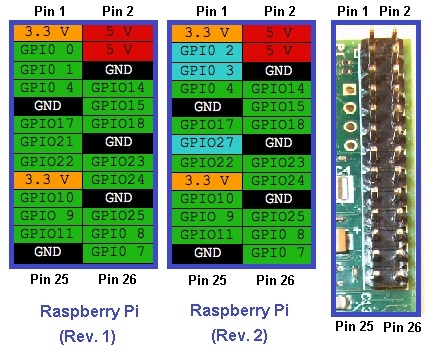
\includegraphics[scale=.6]{GPIO/images/PiA}}\hspace{2cm}
	\subfloat[Model 40 pin GPIO]
	{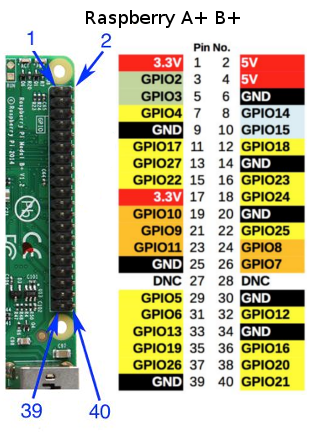
\includegraphics[scale=.6]{GPIO/images/PiB}}
%\end{center}
\caption{Số chân GPIO của các phiên bản Raspberry Pi}\label{Fig:gpio}
\end{figure}
\section{Mô tả chức năng của các nhóm chân}
Trên Raspberry Pi sẽ có các nhóm chân sau đây (ta sẽ sử dụng cách đánh số từ $1 \rightarrow 40$ như trên hình \ref{Fig:gpio}):
\begin{itemize}
\item \textit{Nhóm chân cấp nguồn:}
\begin{itemize}
\item Nguồn 5V: gồm 2 chân -- số 2 và 4.
\item Nguồn 3.3V: gồm 2 chân -- số 1 và 17.
\item Chân GND: gồm 5 chân -- số $6,9,14,25$ (Model 26 chân) hoặc gồm 8 chân -- số $6,9,14,25,30,$ $34,39$ (Model 40 chân).
\end{itemize}
\item \textit{Nhóm chân GPIO (I/O):}
\begin{itemize}
\item Model 26 chân: gồm 8 chân -- số $7, 11, 12, 13, 15, 16, 18, 22$.
\item Model 40 chân: gồm 17 chân -- số $7, 11, 12, 13, 15, 16, 18, 22, 29, 31, 32, 33, 35, 36,$ $37, 38, 40$.
\end{itemize}
\item \textit{Chân PWM -- Pulse Width Modulation}: gồm 2 chân -- chân số 12 và 13.
\item \textit{Nhóm chân giao tiếp $I2C$}: gồm 2 chân -- số 3 và 5.\\
Ta có thể điều khiển nhiều thiết bị I2C chỉ với 2 chân này, mỗi thiết bị sẽ được phân biệt bởi một địa chỉ riêng của nó. Cần khai báo đúng địa chỉ của thiết bị cần điều khiển.
\item \textit{Nhóm chân giao tiếp $SPI$:} gồm 5 chân -- số $19, 21, 23, 24, 26$.
\item \textit{Nhóm chân giao tiếp UART}: gồm 2 chân -- số 8 và số 10.
\item \textit{Nhóm chân giao tiếp EEPROM:} gồm 2 chân -- số 27 và 28 (chỉ có ở model Pi có 40 chân GPIO).
\end{itemize}
\section{Các cài đặt và cấu hình cần thiết để sử dụng được các chân GPIO}
Trong bài viết mình sẽ chọn ngôn ngữ lập trình Python (Phython 2) để điều khiển các chân GPIO của Raspberry Pi. Những dọng lệnh bên dưới, sẽ được thực hiện trên của sổ dòng lệnh.
\subsection{Cài đặt thư viện RPi.GPIO}
Gõ lệnh sau: \verb|sudo apt-get install python-dev python-rpi.gpio|
\subsection{Xác nhận cấu hình I2C}\label{Sub:I2C}
Chỉ khi nào giao tiếp I2C thì mới thực hiện \textit{mục \ref{Sub:I2C}}.

Gõ lệnh sau: \verb|sudo apt-get install python-smbus i2c-tools|

Chạy \verb|sudo raspi-config| để Enable I2C (thường khi cài đặt hệ điều hành thì I2C ở chế độ Disable).

Thực hiện theo các bước từ \textit{hình \ref{Fig:start}} đến \textit{hình \ref{Fig:reset}} trong \textit{hình \ref{Fig:I2C}}. Sau khi thực hiện bước cuối cùng trong \textit{hình \ref{Fig:reset}}, Raspberry Pi sẽ reset lại.
\begin{figure}
	\subfloat[Chọn \textsf{8 Advance Options} rồi \textsf{Enter}\label{Fig:start} ]
	{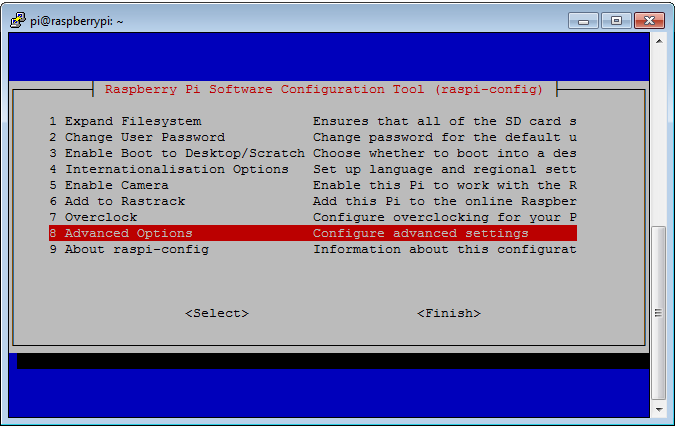
\includegraphics[scale=.45]{GPIO/images/raspi-1}}\hspace{1cm}
	\subfloat[Chọn \textsf{A7 I2C} rồi \textsf{Enter}\label{Fig:b2}]
	{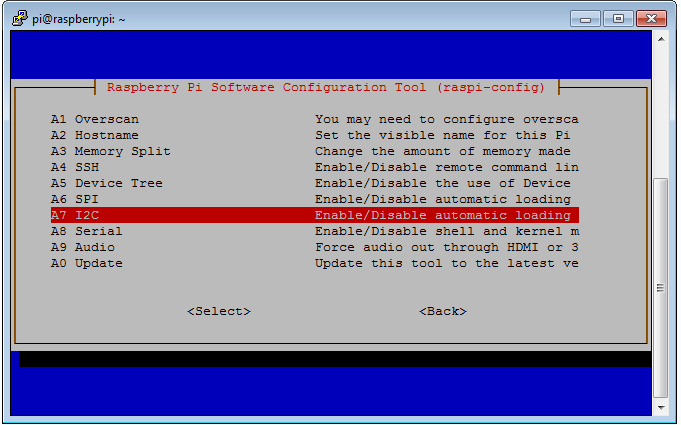
\includegraphics[scale=.45]{GPIO/images/raspi-2}}\\
	\subfloat[Chọn \textsf{Yes} rồi \textsf{Enter}]
	{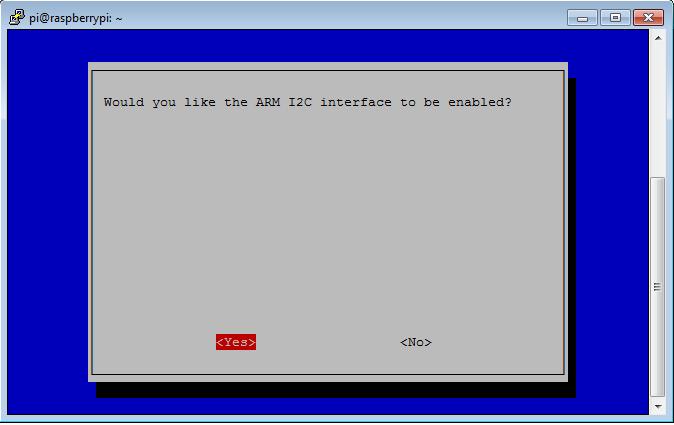
\includegraphics[scale=.45]{GPIO/images/raspi-3}}\hspace{1cm}
	\subfloat[Chọn \textsf{OK} rồi \textsf{Enter}]
	{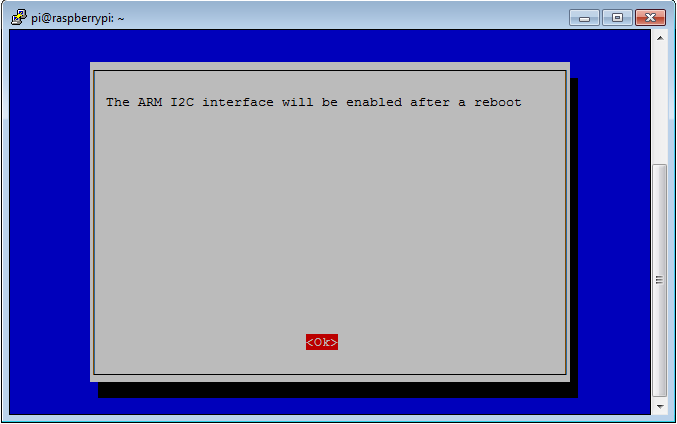
\includegraphics[scale=.45]{GPIO/images/raspi-4}}\\
	\subfloat[Chọn \textsf{Yes} rồi \textsf{Enter}]
	{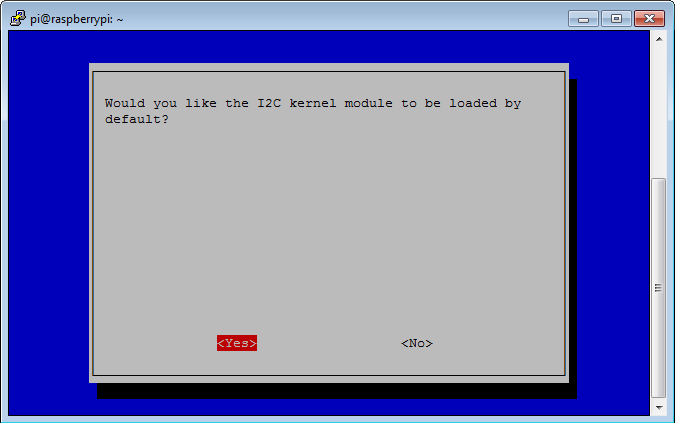
\includegraphics[scale=.45]{GPIO/images/raspi-5}}\hspace{1cm}
	\subfloat[Chọn \textsf{OK} rồi \textsf{Enter}]
	{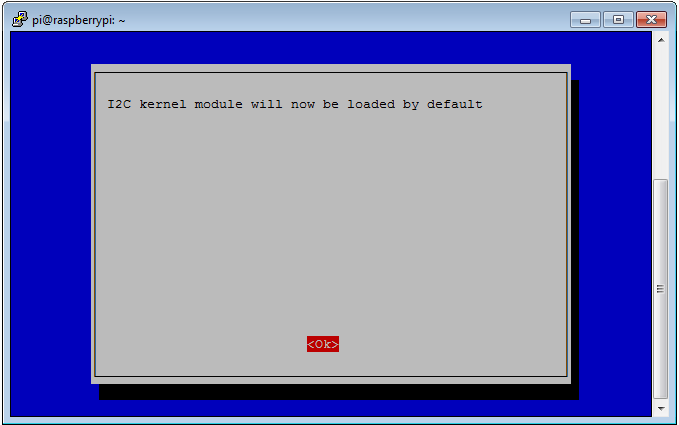
\includegraphics[scale=.45]{GPIO/images/raspi-6}}\\
	\subfloat[Chọn \textsf{Finish} rồi \textsf{Enter}]
	{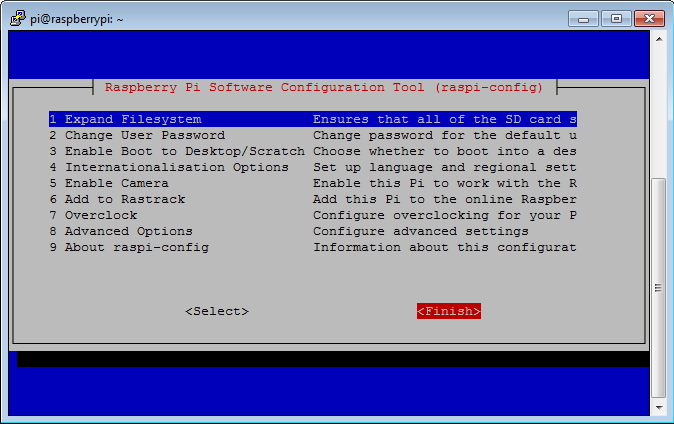
\includegraphics[scale=.45]{GPIO/images/raspi-7}}\hspace{1cm}
	\subfloat[Chọn \textsf{Yes} rồi \textsf{Enter}\label{Fig:reset}]
	{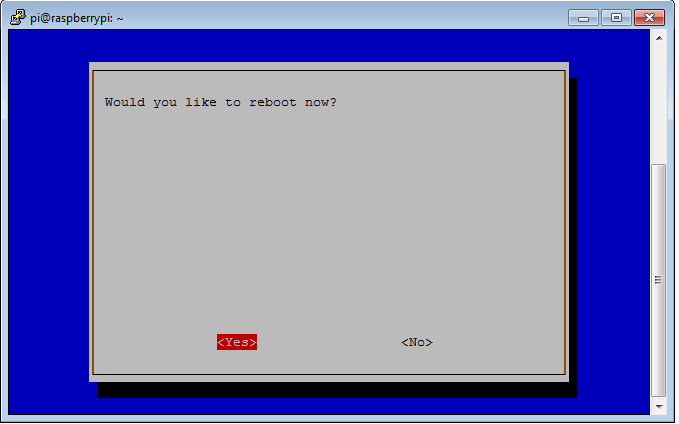
\includegraphics[scale=.45]{GPIO/images/raspi-8}}\\
	
\caption{Cách cấu hình I2C trên Raspberry Pi} \label{Fig:I2C}
\end{figure}
Khi Raspberry Pi khởi động trở lại, ta thực hiện, tiếp:
\begin{itemize}
\item Mở file \verb|modules|, dùng lệnh: \verb|sudo nano /etc/modules|
\item Thêm vào file \verb|moludes| với nội dụng giống như hình bên dưới: thêm vào 2 dòng \verb|i2c-bcm2708| và \verb|i2c-dev| (Nhấn Ctrl + X + Y để lưu file và thoát khỏi).
\begin{figure}[!h]
\begin{center}
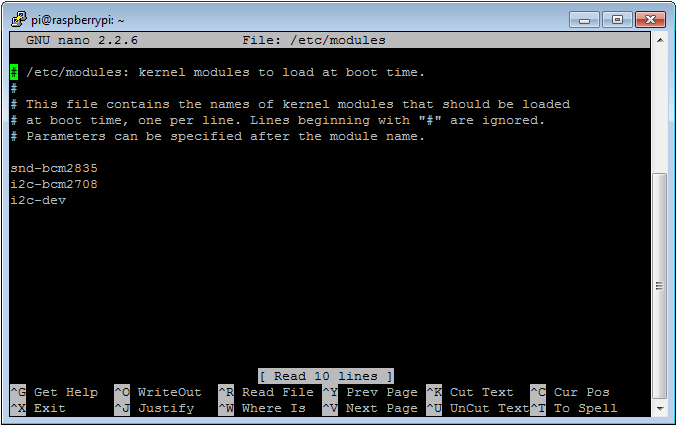
\includegraphics[scale=.5]{GPIO/images/raspi-9}
\end{center}
\end{figure}
\item Mở file \verb|raspi-blacklist.conf|, dùng lệnh:
\begin{center}
\verb|sudo nano /etc/modprobe.d/raspi-blacklist.conf|
\end{center}
\item Thêm dấu \verb|#| vào trước 2 dòng: \verb|blacklist spi-bcm2708| và \verb|blacklist i2c-bcm2708| (Nhấn Ctrl + X + Y để lưu file và thoát khỏi).
\begin{figure}[!h]
\begin{center}
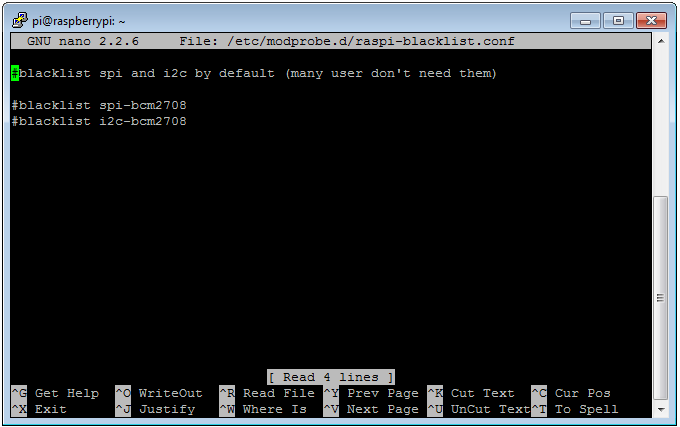
\includegraphics[scale=.5]{GPIO/images/raspi-10}
\end{center}
\end{figure}
\item Sau khi thực xong, chúng ta reset lại Raspberry Pi: \verb|sudo reboot|
\end{itemize} 
\subsection{Xác nhận cấu hình SPI}\label{Sub:SPI}
Chỉ khi nào giao tiếp SPI thì mới thực hiện \textit{mục \ref{Sub:SPI}}.\\

Thực hiện \verb|Enable| SPI với lệnh \verb|sudo raspi-config|, tương tự như \verb|Enable| I2C (đến \textit{hình \ref{Fig:b2}} ta chọn \verb|A6 SPI|).\\

Khi Raspberry Pi khởi động trở lại, ta thực hiện:
\begin{itemize}
\item Mở file \verb|raspi-blacklist.conf|, dùng lệnh:
\begin{center}
\verb|sudo nano /etc/modprobe.d/raspi-blacklist.conf|
\end{center}
\item Thêm dấu \verb|#| vào trước 2 dòng: \verb|blacklist spi-bcm2708| và \verb|blacklist i2c-bcm2708| (Nhấn Ctrl + X + Y để lưu file và thoát khỏi). Nếu không có file này thì hãy tạo lại với nội dung như bên dưới.
\end{itemize}
\section{Sử dụng các chân GPIO để điều khiển phần cứng cùng với ngôn ngữ lập trình Python}
Phần này dựa vào bài viết của tác giả: \textsf{Anonymous} với chủ đề:

\textit{raspberry-gpio-python -- A Python module to control the GPIO on a Raspberry Pi} \footnote{\textsf{https://sourceforge.net/p/raspberry-gpio-python/wiki/Examples/}}\\

Hiện tại thì thư viện này chưa hổ trợ các giao tiếp SPI, I2C, 1-wire, chúng ta chỉ sử dụng nó với các lệnh cơ bản bên dưới.

Tránh đặt điện áp lớn hơn 3.3V vào trực tiếp các chân GPIO vì sẽ làm hỏng chúng.
\subsection{Kiểm tra chức năng của các chân GPIO}
Sử dụng các chân GPIO trên Raspberry Pi phải đúng với chức năng của nó thì mới đem lại hiệu quả.
\begin{itemize}
\item Kiểm tra chức năng của từng chân:
\begin{lstlisting}[language=Python]
import RPi.GPIO as GPIO

GPIO.setmode(GPIO.BOARD)
func = GPIO.gpio_function(pin)
\end{lstlisting}
\item Kết quả trả về là: \verb|GPIO.IN|, \verb|GPIO.OUT|, \verb|GPIO.SPI|, \verb|GPIO.I2C|, \verb|GPIO.HARD_PWM|, \verb|GPIO.SERIAL|, \verb|GPIO.UNKNOWN|
\end{itemize}
\subsection{Các lệnh cơ bản trong thư viện RPi.GPIO}
%\lstinputlisting[language=Python]{import.py}
\begin{itemize}
\item Khai báo thư viện \verb|RPi.GPIO|:
\begin{lstlisting}[language=Python]
import RPi.GPIO as GPIO #Dung ten GPIO thay cho RPi.GPIO
\end{lstlisting}
Kiểm tra thông tin về Pi và chân GPIO:
\begin{lstlisting}[language=Python]
GPIO.RPI_INFO
#Ket qua tra ve: P1_REVISION; RAM; REVISION; TYPE; PROCESSOR; MANUFACTURER
#Vi du: {'P1_REVISION': 3, 'RAM': '512M', 'REVISION': '0010', 'TYPE': 'Model B+', 'PROCESSOR': 'BCM2835', 'MANUFACTURER': 'Unknown'}
#Ta co the dung lenh: GPIO.RPI_INFO[Tham so] de xem mot thong so quan tam

#Dung lenh: GPIO.RPI_REVISION de xem phien ban chan GPIO 
GPIO.VERSION #Kiem tra phien ban GPIO
#Vi du: '0.6.2'
\end{lstlisting}
\item Xác định cách khai báo số chân là \verb|GPIO.BOARD| hay \verb|GPIO.BCM|:
\begin{lstlisting}[language=Python]
GPIO.setmode(GPIO.BOARD) #Danh so chan theo so tren Board tu so 1 den so 40
GPIO.setmode(GPIO.BCM) #Danh so chan theo ten GPIO, vi du GPIO27, GIPO14,...
\end{lstlisting}
Để kiểm tra xem bạn đang sử dụng cách khai báo nào trong 2 cách khai báo \verb|BOARD| hoặc \verb|BCM|, dùng lệnh sau:
\begin{lstlisting}[language=Python]
mode = GPIO.getmode() #Xem khai bao BOARD hoac BCM
print mode  
#mode = -1: chua khai bao
#mode = 10: khai bao la BOARD
#mode = 11: khai bao la BCM
\end{lstlisting}
\item Khi các chân GPIO đã được sử dụng trước đó (chưa được cleanup) thì sử dụng lại chương trình sẽ thông báo các cảnh báo, ta sử dụng lệnh sau để vô hiệu cảnh báo:
\begin{lstlisting}[language=Python]
GPIO.setwarnings(False) #Bo qua cac canh bao ve GIPO
\end{lstlisting}
\item Khai báo chân GPIO cần điều khiển là chân \verb|input| hay chân \verb|output|:
\begin{lstlisting}[language=Python]
#pin la chan GPIO can dieu khien
GPIO.setup(pin, GPIO.IN) #Khai bao pin chan INPUT
GPIO.setup(pin, GPIO.OUT) #Khai bao pin chan OUTPUT


#Khi can khai bao nhieu chan INPUT va OUTPUT
pin_input = [pin1, pin2, pin2] #Danh sach cac chan INPUT
pin_output = [pin4, pin4, pin6] #Danh sach cac chan OUTPUT

GPIO.setup(pin_input, GPIO.OUT) #Khai bao nhieu chan la INPUT
GPIO.setup(pin_output, GPIO.OUT) #Khai bao nhieu chan la OUTPUT
\end{lstlisting}
\item Với một số ứng dụng ta cần \textit{mắc điện trở treo (lên nguồn hoặc nối mass)}: có thể làm việc này bằng phần cứng hoặc bằng phần mềm. Ở đây ta sử dụng phần mềm.
\begin{lstlisting}[language=Python]
#pin1, pin2 la chan GPIO can dieu khien

#Khai bao pin chan INPUT, co dien tro mac len nguon - 3.3V
GPIO.setup(pin1, GPIO.IN,pull_up_down = GPIO.PUD_UP) 

#Khai bao pin chan INPUP, co dien tro mac xuong mass - 0V
GPIO.setup(pin2, GPIO.IN, pull_up_down = GPIO.PUD_DOWN) 
\end{lstlisting}
\item Đọc tín hiệu từ chân \verb|INPUT|:
\begin{lstlisting}[language=Python]
#pin la chan GPIO can dieu khien
read_input = GPIO.input(pin) #Doc tin hieu cua chan INPUT
#read_input la 0 hoac 1 hoac GIPO.LOW hoac GPIO.HIGH hoac False hoac True
\end{lstlisting}
\item Xuất tín hiệu ra chân GPIO là chân \verb|OUTPUT|:
\begin{lstlisting}[language=Python]
#pin la chan OUTPUT

#Co 3 cach xuat chan GPIO pin ra muc cao
GPIO.output(pin,1)
GPIO.output(pin,True) 
GPIO.output(pin,GPIO.HIGH) 

#Co 3 cach xuat chan GPIO pin ra muc thap
GPIO.output(pin,0)
GPIO.output(pin,False) 
GPIO.output(pin,GPIO.LOW)

#Khi can xuat tin hieu ra nhieu chan
pin_output = [pin1, pin2, pin3] #Danh sach cac chan OUTPUT
GPIO.output(pin_output,0) #Cac pin o muc thap, 
GPIO.output(pin_output,0) #Cac pin o cao
#Co the su dung tham so: 0, 1 hoac False, True hoac GPIO.LOW, GPIO.HIGH 

#Ham Output va Input ket hop voi nhau
#Doc gia tin hieu tu 1 chan va xuat no ra chinh no pin
GPIO.output(pin, not GPIO.input(pin))
\end{lstlisting}
\item Kết thúc quá trình làm việc với các chân GPIO, có 2 tùy chọn:
\begin{lstlisting}[language=Python]
GPIO.cleanup() #clear tat ca cac chan GPIO
GPIO.cleanup([pin_1, pin_2]) #Chi clear mot so chan GPIO
\end{lstlisting}
\end{itemize}
\subsection{Ngắt và phát hiện tín hiệu cạnh}
\textit{Ngắt} là bắt chương trình dừng công việc đang thực hiện để thực hiện một công việc khác.

\textit{Tín hiệu cạnh} là tín hiệu số biến đổi từ mức thấp lên mức cao ($0 \rightarrow 1$) hoặc từ mức cao xuống mức thấp ($1 \rightarrow 0$).
\begin{itemize}
\item Hàm \verb|wait_for_edge()|: thực hiện chương trình khi phát hiện được tín hiệu cạnh.
\begin{lstlisting}[language=Python]
#Phat hien tin hieu canh o chan GPIO pin
GPIO.wait_for_edge(pin, GPIO.RISING)  #RISING chuyen tu 0 len 1
GPIO.wait_for_edge(pin, GPIO.FALLING)  #FALLING chuyen tu 1 xuong 0
GPIO.wait_for_edge(pin, GPIO.BOTH)  #BOTH chi can co tin hieu canh
#GPIO.BOTH gom GPIO.RISING va GPIO.FALLING

#Khi can doi tin hieu canh trong thoi gian nhat dinh
#Doi tin hieu canh (RISING,FALLING, BOTH) trong thoi gian timeout = t
#Don vi cua t la ms, vi du: timeout = 5000 (t = 5s)
#Neu qua thoi gian timeout ma khong phat hien canh thi ket qua la None

#Doi canh chuyen tu 0 len 1 voi thoi gian t (ms)
signal_edge  = GPIO.wait_for_edge(pin, GPIO.RISING, timeout=t) 

#Doi canh chuyen tu 1 len 0 voi thoi gian t (ms)
signal_edge  = GPIO.wait_for_edge(pin, GPIO.FALLING, timeout=t) 

#Doi tin hieu canh voi thoi gian t (ms)
signal_edge  = GPIO.wait_for_edge(pin, GPIO.BOTH, timeout=t) 
\end{lstlisting}
\item Hàm \verb|event_detected()|: khi chương trình đang thực hiện một công việc nào đó, nếu có tín hiệu cạnh thì nó sẽ nhảy sang một việc khác.
\begin{lstlisting}[language=Python]
GPIO.add_event_detect(pin, GPIO.RISING) #FALLING, BOTH
#Phat hien tin hieu canh tu 0 len 1
#
#Cong viec dan thuc hien vi du: trong vong lap for, while,...
#
if GPIO.event_detected(channel):
	print "Thuc hien chuong trinh o phan nay"
\end{lstlisting}
\item Dùng chức năng phát hiện cạnh thì nhảy sang \textit{chương trình ngắt} được định nghĩa trước để thực hiện câu lệnh.
\begin{lstlisting}[language=Python]
def chuong_trinh_ngat_1():
	#
	#Noi dung can thuc hien khi co ngat
	#

def chuong_trinh_ngat_2():
	#
	#Noi dung can thuc hien khi co ngat
	#
GPIO.add_event_detect(pin, GPIO.RISING) #FALLING, BOTH
GPIO.add_event_callback(pin, chuong_trinh_ngat_1())
GPIO.add_event_callback(pin, chuong_trinh_ngat_2())

#Them vao tham so bouncetime = t(ms) de chong nhieu
GPIO.add_event_callback(pin, chuong_trinh_ngat_1, bouncetime=t)
GPIO.add_event_callback(pin, chuong_trinh_ngat_2, bouncetime=t)
\end{lstlisting}
\item Hàm \verb|remove_event_detect()|: không sử dụng chức của hàm \verb|event_detected()| nữa.
\begin{lstlisting}[language=Python]
GPIO.remove_event_detect(pin) #pin GPIO duoc su dung voi ngat truoc do
\end{lstlisting}
\end{itemize}
\subsection{Sử dụng chân GPIO với chức năng PWM}
Ta thực hiện theo các bước:
\begin{itemize}
\item Khởi tạo một khối PWM:
\begin{lstlisting}[language=Python]
p = GPIO.PWM(channel, freq)
#channel: chan so 12 va so 13 hoac GPIO18 va GPIO27
#freq: tan so xung vuong
\end{lstlisting}
\item Bắt đầu với PWM:
\begin{lstlisting}[language=Python]
p.start(duty_cycle)
#duty_cycle = T_on/T = T_on/(T_on T_off) = 0 - 100%
\end{lstlisting}
\item Lệnh thay đổi tần số và chu kỳ:
\begin{lstlisting}[language=Python]
#Thay doi tan so
p.ChangeFrequency(freq) #freq: la tan so moi

#Thay doi phan tram T_on
p.ChangeDutyCycle(duty_cycle) #duty_cycle: phan tram T_on moi
\end{lstlisting}
\item Dừng khối PWM:
\begin{lstlisting}[language=Python]
p.stop() #Dung khoi PWM voi ten bien la p
\end{lstlisting}
\end{itemize}
%\subsection{Các lệnh trong thư viện RPi.GPIO}
\end{document}